\section{Benchmarks for Selected DBMS:s} \label{sec:benchmarks}
Source and how to reproduce benchmark results: \cite{benchmark}
\begin{figure}[h] % "h" means "here"
    \centering
    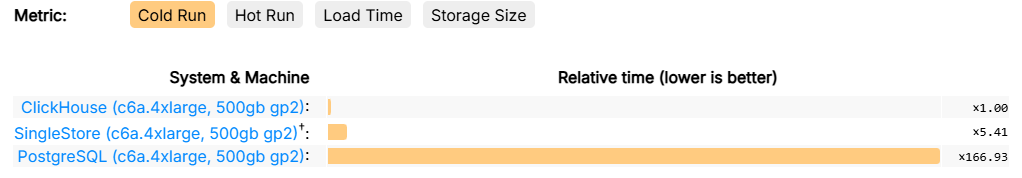
\includegraphics[width=1.0\textwidth]{Figures/Q7_bench_crun.PNG}
    \label{fig:Cold run benchmark}
    \caption{Cold run benchmark} % Add caption
\end{figure}

\begin{figure}[h] % "h" means "here"
    \centering
    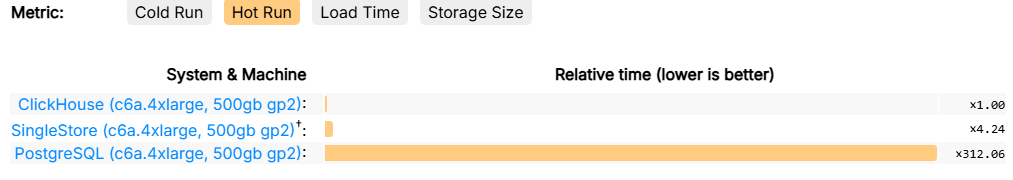
\includegraphics[width=1.0\textwidth]{Figures/Q7_bench_hrun.PNG}
    \label{fig:Hot run benchmark}
    \caption{Hot run benchmark} % Add caption
\end{figure}


\begin{figure}[h] % "h" means "here"
    \centering
    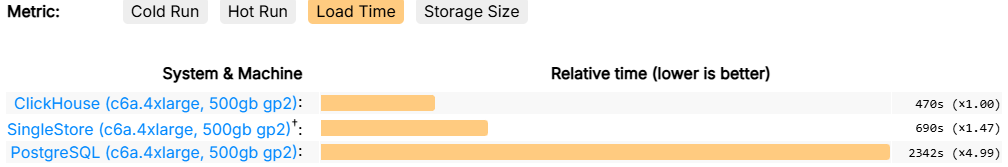
\includegraphics[width=1.0\textwidth]{Figures/Q7_bench_loadT.PNG}
    \label{fig:Load time benchmark}
    \caption{Load time benchmark} % Add caption
\end{figure}


\begin{figure}[h] % "h" means "here"
    \centering
    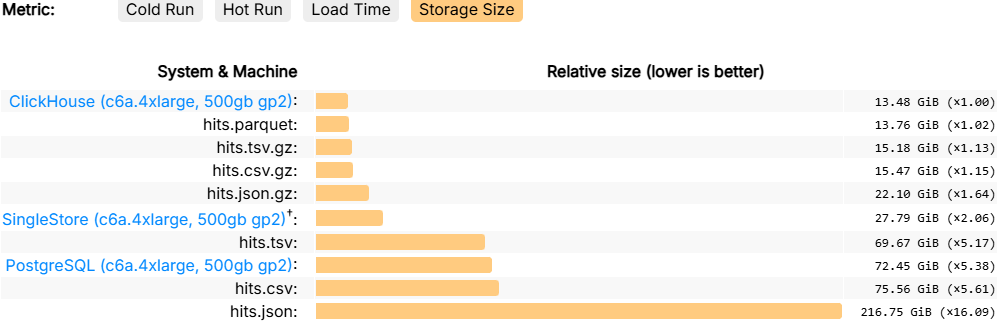
\includegraphics[width=1.0\textwidth]{Figures/Q7_bench_storageS.PNG}
    \label{fig:Storage size benchmark}
    \caption{Storage size benchmark} % Add caption
\end{figure}

\newpage

\section{Interview Transcript} \label{sec:interview}
\begin{quote}
    \textbf{Interviewer:} What is the value of data warehouse decision-making in your organization?
    
    \textbf{Interviewee:} well at our place we use um our we don't strictly use the data warehouse but rather data lakehouse and our data platform provides quite a lot of value when it comes to decision making.

    We use it for things like finance, health and safety, sales, marketing and yeah a bunch of other different places... It's a little bit case by case basis but you know we're
    a housing development company so one instance would be that the project leads for any of our housing projects they have a continuously updated report where they can track the economics and the health and safety and all of the things that they need to be on top of to see how things are developing with their projects
    
    And this kind of enables them to see the data see trends, if we're having cost overruns what part of the construction project is it happening in and is there any way to
    you know make this cost go away. That's one case. 
    Same thing with our marketing people they use this to track where they spend the money, what are the returns on investment by marketing different channels, this helps them to evaluate each campaign they drive through, and at the end of the day they can look at what what did they put in what did they get out and they can decide if they want to move to making the next smart campaigns in other areas or if they'd rather continue more in the same area.
    
    Or for instance if you want to do your ads on Google or Youtube.
    
    Same thing with sales our whole sales pipeline is very connected to... we have a CRM system of course like everyone else does but everything is aggregated connected to and aggregated to our data platform or rather connected to and aggregated within our data platform.
    
    So we can look at more of the overarching trends for sales and see what projects are we building where sales are going slow where are they going quickly.
    And these things are great both to see what projects we have which would need more love in the sales and where we could put more effort into getting these units sold, because having an empty apartment for any stretch of time is a waste of money.
    But in the same way this can also be used retroactively at the larger scale to look at what type of projects has turned out to be very lucrative and also what has turned out to be very hot on the market and make evaluations on maybe we're underpricing things if we sell at a very high pace, or maybe we're overpricing things if we sell things at a too slow pace.
    
    Same thing. I don't know. You want me to keep coming up with examples or...

    \textbf{Interviewer:} No thank you, that should be sufficient.

    \textbf{Interviewee:} Good to hear.

    \textbf{Interviewer:} Next question then, Which decisions could be supported via the data warehouse?

    \textbf{Interviewee:} Well, so as I mentioned before, we are already using it for decision support to quite an extent. But we're mostly working with our own data. And one of the directions we've started looking at and trying to figure out is how can we incorporate more external data than we are today, and look at things like, how is the housing market doing in general? What are current trends on you know, with construction work and housing development? What kind of trends are we seeing in general with marketing? And just this kind of work with incorporating data from a much broader range of sources, and trying to incorporate those in our analysis, those, I think would be something which we could support, which we don't do as of yet.

    \textbf{Interviewer:} Great, thank you. And machine learning, what do you think could be useful there?

    \textbf{Interviewee:} Yeah, I think that's a very good question.I think we could use machine learning for a couple of different use cases. One which is very strong, but maybe a bit boring is automation and efficiency. Because we just as every organization, or every person on this planet, we have a bunch of repetitive tasks. And we can use machine learning to automate them. We already do this for automate automatic categorization of invoices to help out the finance department. And this has been very useful to have the data underlying this, of course. But then I think we could also start looking at machine learning models or other types of advanced analytics to spot patterns in the market and figure out what kind of decisions we should make. And if there's any good predictors for what is going to be a lucrative project or not for us.

    \textbf{Interviewer:} And that's where the external data sources come in as well, I guess.

    \textbf{Interviewee:} Yeah, exactly. Yeah, for machine learning. That's what we'd use the combination of our own and external data, of course.

    \textbf{Interviewer:} Okay, thank you. Next question then. What is the role of analytics sandboxes in today's business intelligence environment?

    \textbf{Interviewee:} Well, so I'm speaking in a bit of an odd position here, because we don't strictly speaking, have an analytic sandbox.

    We at because we work with a quite flexible system from the get go, as opposed to data warehouse we work with a data lakehouse.
    
    And we also all of our code is in Spark, and all of our data is stored in (Apache) Parquet files.
    
    So, but with that said, we do have a development test and production environment more like software developers would do it. 
    And with this we have a development environment where we can do... either we can create artificial or hypothetical data to try out some kind of hypothesis with our current analysis versions, or we can look at current like real current data and try new analysis methods, or we can do any combination of them.
    And we're connected to all the different data sources in their environments as well so we can take in hypothetical data which is created in other systems so we have a lot of flexibilities in the ways we work which I think is what you want to get out of an analytic sandbox.
    
    And this is great for us because we can both... we can very quickly develop and we can try out new features at a high pace without having to modify our production environment and we can actually be very fearless in our work and we can move rapidly and this is one of the main points for us at least and i think for anyone using an analytic sandbox.
    Other than that we do have like the tool we work with for all of our calculations and transformations generally is Spark.
    
    And one of the main perks with Spark is that it's very very flexible in how you want to work with it. 
    For example, all of our automatically running transformations in pipelines we work with with Spark jobs which is more like a script and they're very rigid we you know we develop them we move them through our different environments we test them we publish them.
    But on the other hand you can just as well use Spark with something called the Notebook and that is very much made for an \textit{ad hoc} analysis so you get great performance because Spark is distributed but you can very very rapidly work your way through problems and you have a very good integration between writing code but also visualizing it in a super helpful way so that's that's probably the most sandboxy thing we do.

    \textbf{Interviewer:} Okay, great. Thank you. So, to understand it a bit, what you're trying to say, in part at least, is that analytical sandboxes can help a lot with what's called ad hoc questions and such things?

    \textbf{Interviewee:} yeah I'd say they're good both for trying out things and developing things which are gonna at some point be less of an \textit{ad hoc} situation, just as well, every now and then the business needs some kind of quick analysis for something super specific where we're gonna do this one time and then doing this kind of analytic sandbox solution where you can just throw it out there see the numbers and see what they return that is super helpful as well definitely.

    \textbf{Interviewer:} Thank you. Last question then, how to select an OLAP tool?

    \textbf{Interviewee:} Yes, very good question. So at our company my team which is the data team we don't really work with an OLAP tool we do have a different team who does work with the OLAP tool i think would be a multi-dimensional one and i think they've selected it on a number of different things.

    One of the main things I know when they got it was performance. It loads the entire data, all the data that it works with, is stored in memory instead of on disk which obviously gives you very good performance benefits, and it's great for looking at high dimensionality data. 
    But i know they've had some issues with the costs getting away quite quickly because everything is in the memory and not on disk...
    
    And another part which I think if I was in charge of selecting an OLAP tool I'd probably look a lot at the kind of development operations regarding it and see that you can work with it in more of the software development ways where you do agile development you have \textbf{CI/CD} (continuous integration/continuous delivery) you work with version control because these things have been a challenge from the get-go for them.
    
    But my team on the other hand we do some of the same things you would do in an OLAP tool and yeah maybe I should mention that at there is currently an ongoing investigation going for phasing out the OLAP tool we currently use at my company.

    \textbf{Interviewer:} the MOLAP tool?

    \textbf{Interviewee:} yeah the multi yeah exactly.

    What we do instead is i think for some of the use cases where you use an OLAP tool of the Spark and notebooks for that kind of quick analysis, moving through the data, trying to figure it out, seeing how it works.
    That on one hand is solved there mostly for us.
    And then on the other hand, the kind of ease of use, nice visualizations, being able to as a kind of end user or a business user for us, they can go through our data and look at it through something like Power BI, which is, it's mostly two dimensional flat, but it's very good given that we, you know, help them, we make nice data sets where everything is reasonably structured.
    You can move through the data and look, you can go up and drill up, drill down, you can do slicing and you can do all of these things to explore the data in there in an easy to use fashion, while not going the full extent, not having something as heavy as an OLAP tool, maybe.

    \textbf{Interviewer:} okay, so it's almost an OLAP cube but not fully...?

    \textbf{Interviewee:} Yeah, I think, I think we have, let's call it a OLAP square in Power BI.
    At least that's the way we use it.
    It could possibly be that you can represent data in more higher dimensionality, but the way we work with it is with two dimensional data.

    \textbf{Interviewer:}So what do you use Power BI for since that's like your pseudo-OLAP tool if I understand that correctly? It's like what you use instead of an OLAP tool so to say.

    \textbf{Interviewee:} So we use it kind of on two ends of the spectrum.
    We have some reports, which we ourselves, we design them and we make them kind of as a ready to use pre-configured, all the metrics are there, all the charts are there. 
    And then the end users, which, you know, might be anyone in the marketing or health and safety or finance department, they get just a continuously updated report where they can navigate around and do some, they can work, they can, you know, they can still drill up, drill down and slice stuff, but it's quite predefined.
    But on the other hand, more within the team and for some of the more power users, we use it so they can pull in slightly rawer data and they can structure it and go through it and kind of explore; data exploration I would probably say it would be the more internal use for the more power users, but while still being a no code environment where you can do kind of drag and drop analysis, I guess you could call it.

    \textbf{Interviewer:}Okay, so when it comes to how to select an OLAP tool in your organization it seems like if there's somewhat of a focus on it being easy to interact with without there being too much of a technolgical barrier?

    \textbf{Interviewee:}Yeah, it should be without too big of a technological barrier.
    It should be, we try to make it so that we do the more heavy lifting and all those things are on the data engineering side and in the data lake house with Spark.
    And then we produce nice data which can be interacted with in a friendly user interface through something like Power BI.
    And I think for us, it works very well.
    But that, again, has a lot to do with us doing a lot of the heavy lifting before getting the data into Power BI
    and having really nice data, which is all quite often,
    we already aggregate some of the data that needs aggregation.
    We filter out all of the data, which definitely should not go in there.

    \textbf{Interviewer:}And you think the tools in Power Bi are sufficient for your use-case or do you think it is lacking in some way?

    \textbf{Interviewee:}I think for us, it works very well. But that again has to do with us doing a lot of the heavy lifting before getting the data into Power Bi. And having really nice data which is quite often already aggregated and filtered. So for our use case, I think it's perfect.
    But if you worked somewhere where you had a data platform which couldn't do as much of the heavy lifting and was more of a just storage place for your data,
    then I think you would need to have something a bit more powerful than, say, Power BI, because it gets bogged down once you get to, it doesn't have the performance of, for instance, our old OLAP tool where you can just put in very large amounts of data and peruse through it anyway you want.
    If you want something like Power BI, you have to be a little bit more careful, I'd say.
    But for us, perfect.

    \textbf{Interviewer:}Okay, okay, and do you know what OLAP tool you're using or you can't say perhaps?

    \textbf{Interviewee:} I am not sure I can say.

    \textbf{Interviewer:} Okay, well, that's okay, that's okay, that's fine.

    \textbf{Interviewee:} But it's one of the big ones.

    \textbf{Interviewer:} Okay, yeah, that's great. Okay, well, thank you very much. That's all the questions. Thank you for taking part in the interview.

    \textbf{Interviewee:} Again, no worries.

\end{quote}